\documentclass[11pt,italian]{article}
\usepackage[T1]{fontenc}
\usepackage[utf8]{inputenc} %utf8 % lettere accentate da tastiera
\usepackage[italian]{babel} % lingua del documento
\usepackage{blindtext}
\usepackage{enumitem}
\usepackage{float}
\usepackage{xcolor}   % for \textcolor
\usepackage[font=small,labelfont=bf,skip=10pt]{caption}
\usepackage{subcaption}
\setlength{\belowcaptionskip}{5pt}
\usepackage{listings}
\lstset{
  basicstyle=\ttfamily,
  columns=fullflexible,
  frame=single,
  breaklines=true,
  postbreak=\mbox{\textcolor{red}{$\hookrightarrow$}\space},
}
\usepackage{hyperref}
\usepackage{cleveref}
\usepackage{graphicx}
\graphicspath{ {./images/} }

% Use lstinline as item in description
\makeatletter
\newcommand*{\lstitem}[1][]{%
  \setbox0\hbox\bgroup
    \patchcmd{\lst@InlineM}{\@empty}{\@empty\egroup\item[\usebox0]\leavevmode\ignorespaces}{}{}%
    \lstinline[#1]%
}
\makeatother

\title{Multiple Sequence Alignment (MSA) \\ di sequenze SARS-CoV-2}

\date{A.A.: 2019/2020}

\author{
    \textsc{Edoardo Silva} 816560 \\
    \textsc{Davide Marchetti} 815990
}

\begin{document}
\maketitle

\section{Abstract}
Il lavoro svolto è diviso in 2 parti e il codice in 4 sezioni:
\subsection{Matrice delle variazioni}
Qui si trovano le prime 2 parti del codice: il recupero per intero delle 14 sequenze usate e la lettura dei file di variazione generati in output nella parte1
\begin{lstlisting}[basicstyle=\small\ttfamily,caption=Porzione di ciclo,label=code:Read fasta = [], language = Python]

    reference_id = load_fasta_id(os.path.join('..', '..', 'project-1', 'input', 'reference.fasta'))
    sequence_ids = read_sequence_ids(paths=[
        os.path.join('..', '..', 'project-1', 'input', 'GISAID'),
        os.path.join('..', '..', 'project-1', 'input', 'ncbi'),
    ])
    sequence_ids.insert(0, reference_id)    #insert reference no variations
    
    ...

    clustal_output = load_output('Clustal-NC_045512.2_2020-05-30_16-51.json')
    variations = clustal_output['unmatches'].items()

\end{lstlisting}
\newpage
Infine nella parte 3 del nostro codice generiamo la tabella delle variazioni \textbf{`table.csv'} per variazione, per poi trasporla.

\begin{lstlisting}[basicstyle=\small\ttfamily,caption=Porzione di ciclo,label=code:creation table.csv = [], language = Python]

...

for key, value in variations:
        row = np.zeros(len(sequence_ids))
        indexes.append('C{}'.format(counter))
        for sequence in value['sequences']:
            row[sequence_ids.index(sequence)] = 1
        rows.append(row)
        counter += 1
        
...

trait_matrix = pd.DataFrame(rows, index=indexes, columns=sequence_ids, dtype=bool).transpose()
trait_matrix = phylogeny.reorder_columns(trait_matrix, axis=0, ascending=False)
trait_matrix.to_csv(os.path.join('..', 'output', 'table.csv'))

\end{lstlisting}

%%insert image 'table.csv'%%

\subsection{Albero filogenetico}
La quarta e ultima parte del codice consiste nel ricostrure l'albero filogenetico prendendo l'output del punto 3 e facendo estensivo uso di funzioni create per questo lavoro nel file \textbf{`phylogeny.py'} per:
\begin{enumerate}
	\item generare matrice compatibile con filogenesi perfetta.
	\item assicurarsi che tutto abbia funzionato e non sia più presente matrice proibita.
	\item generare e stampare in output l'albero delle sequenze.
\end{enumerate}
\begin{lstlisting}[basicstyle=\small\ttfamily,caption=Porzione di ciclo,label=code:creation table.csv = [], language = Python]
candidate_matrix = get_perfect_phylogeny_character_matrix(trait_matrix)
if phylogeny.is_forbidden_matrix(candidate_matrix):
        raise Exception('Invalid perfect phylogeny matrix')
phylogeny.build_tree(candidate_matrix)
\end{lstlisting}

%%parte filogenesi perfetta da mettere?%%

La generazione dell'albero viene svolta come segue:
	
\begin{enumerate}
	\item Riordino il dataframe ordinando le colonne per numero decrescende di 1
\begin{lstlisting}[basicstyle=\small\ttfamily,caption=Porzione di ciclo,label=code:1 = [], language = Python]	
    sorted_axis = df.sum(axis=0).sort_values(ascending=False)
    if axis == 0:
        return df[sorted_axis.index]
    return df.reindex(sorted_axis.index)
\end{lstlisting}
	\item Genera nodo radice, poi per ogni sequenza genera nodi da collegare a root se incontra la presenza di variazione per ogni nodo non già presente
	%guarda questa parte
\begin{lstlisting}[basicstyle=\small\ttfamily,caption=Porzione di ciclo,label=code:1 = [], language = Python]	
for i, row in df.iterrows():
        current_node = root

        for j in range(len(row)):
            # If alteration is present in the current sequence
            if row.iloc[j]: #true in cell
                key = j
                # If current_node is already linked to the j-th variation
                # edges = dictionary with links from (current_node, u)
                if key in current_node.edges:
                    # Update the current node
                    current_node = current_node.edges[key]
                else:
                    # Create a new node u and link it with the last node of this sequence
                    u = Node('U-{}'.format(row.index[j]), edges={}, parent=current_node)
                    current_node.edges[key] = u
                    current_node = u
        # We looped all the variations, insert the sequence node at the end of the chain
        Node(i, parent=current_node)	
\end{lstlisting}
\item Conversione dell'albero precedentemente generato in un newick\_tree elaborabile dalla libreria \textbf{Phylo}, usata per la visualizzazione.
\begin{lstlisting}[basicstyle=\small\ttfamily,caption=Porzione di ciclo,label=code:1 = [], language = Python]	
newick_tree = to_newick_tree(root, intermediates=False)
newick_tree = Phylo.read(io.StringIO(newick_tree), 'newick')
\end{lstlisting}
\item Generazione immagine output
\begin{lstlisting}[basicstyle=\small\ttfamily,caption=Porzione di ciclo,label=code:1 = [], language = Python]	
fig = plt.figure(figsize=(10, 8))
    ax = fig.add_subplot(1, 1, 1)

    # Assign sequences data to the leaf
    root = newick_tree.clade
    merge_sequences_data(root, sequences_data) # Add sequence data to sequence leaves
    # Render with plt
    Phylo.draw(newick_tree, do_show=False, axes=ax)

    ax.set_xlabel('Number of alterations')
    ax.set_ylabel('Sequences')
    plt.tight_layout()
    plt.savefig(os.path.join('..', 'output', 'phylogenetic-tree.png'))
    plt.show()
\end{lstlisting}
\end{enumerate}

\section{Confronto alberi}
\begin{figure}[H]
  \makebox[\textwidth][c]{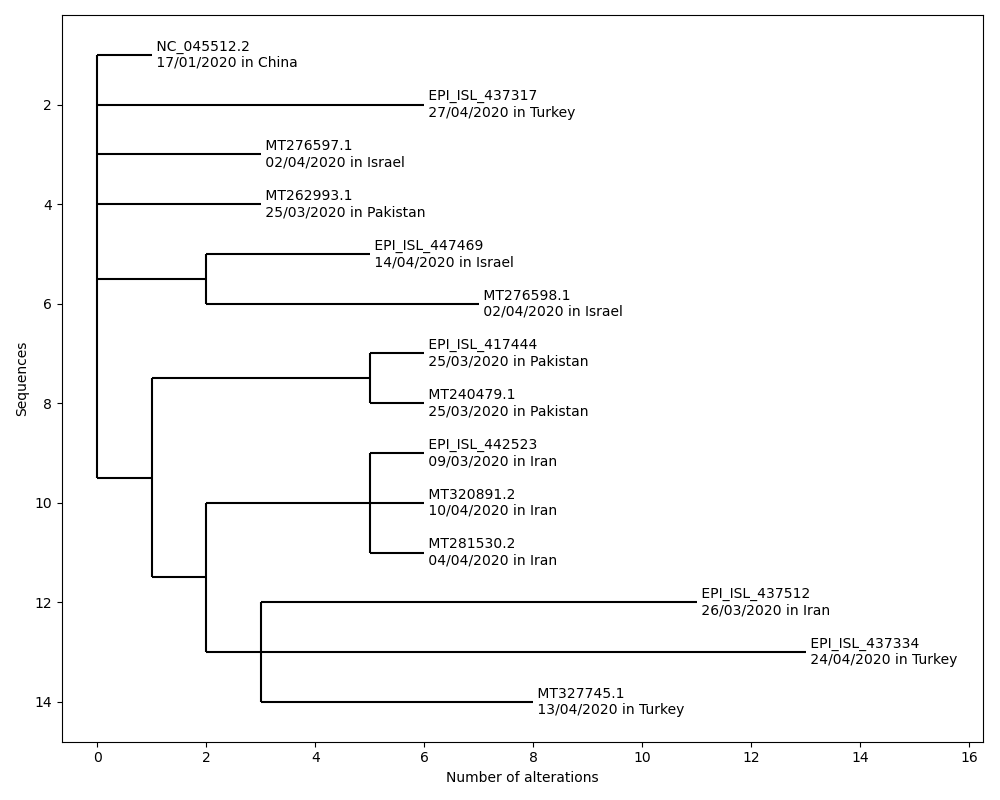
\includegraphics[width=1.3\linewidth]{../output/phylogenetic-tree.png}}
  \caption{Albero di output dello script}
  \label{fig:jalview-end}
\end{figure}
\begin{figure}[H]
  \makebox[\textwidth][c]{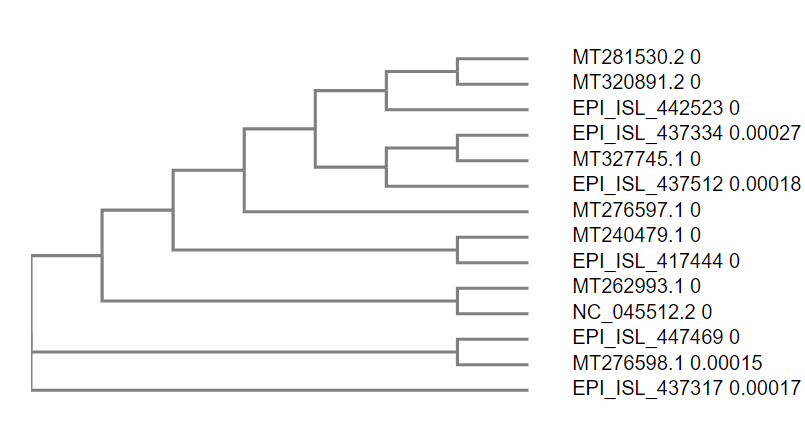
\includegraphics[width=1.3\linewidth]{ncbi_tree.png}}
  \caption{Albero di output del sito delle sequenze}
  \label{fig:jalview-end}
\end{figure}

\section{conclusione}


\end{document}